\documentclass[conference]{IEEEtran}
\IEEEoverridecommandlockouts

% Language setting
% Replace `english' with e.g. `spanish' to change the document language
\usepackage[english]{babel}

% Set page size and margins
% Replace `letterpaper' with `a4paper' for UK/EU standard size
\usepackage[letterpaper,top=2cm,bottom=2cm,left=3cm,right=3cm,marginparwidth=1.75cm]{geometry}

% Useful packages
\usepackage{amsmath}
\usepackage{graphicx}
\usepackage{csquotes}
\usepackage[colorlinks=true, allcolors=blue]{hyperref}
\usepackage[shortlabels]{enumitem}
\usepackage{textcomp}
\usepackage{cleveref}

% Bibliography
\usepackage[
    backend=biber,
    style=ieee,
    natbib,
    mincitenames=1,
    maxcitenames=1,
    uniquelist,
    doi=false,
    url=false,
    sorting=none,
    maxbibnames=10,
]{biblatex}
\addbibresource{sample.bib}
%\addbibresource{bib-leo.bib}

% Acronyms
\usepackage[acronyms]{glossaries}
\newacronym{fl}{FL}{Federated Learning}
\newacronym{ml}{ML}{Machine Learning}
\newacronym{dl}{DL}{Deep Learning}
\newacronym{ids}{IDS}{Intrusion Detection System}
\newacronym{fids}{FIDS}{Federated Intrusion Detection System}
\newacronym{cids}{CIDS}{Collaborative Intrusion Detection System}
\newacronym{ai}{AI}{Artificial Intelligence}
\newacronym{siem}{SIEM}{Security Information and Event Management}
\newacronym{niid}{NIID}{Non Identically or Independently Distributed}
\newacronym{cdfl}{CD-FL}{Cross-Device Federated Learning}
\newacronym{csfl}{CS-FL}{Cross-Silo Federated Learning}

\glsdisablehyper

% Abbreviations
\usepackage{xspace}
\makeatletter
\DeclareRobustCommand\onedot{\futurelet\@let@token\@onedot}
\def\@onedot{\ifx\@let@token.\else.\null\fi\xspace}
\def\eg{\emph{e.g}\onedot} \def\Eg{\emph{E.g}\onedot}
\def\ie{\emph{i.e}\onedot} \def\Ie{\emph{I.e}\onedot}
\def\cf{\emph{cf}\onedot} \def\Cf{\emph{C.f}\onedot}
\def\etc{\emph{etc}\onedot} \def\vs{\emph{vs}\onedot}
\def\wrt{w.r.t\onedot} \def\dof{d.o.f\onedot}
\def\etal{\emph{et al}\onedot}
\makeatother

\makeatletter
\def\paragraph{\@startsection{paragraph}{4}{\parindent}{0ex plus 0.1ex minus 0.1ex}%
{0ex}{\normalfont\normalsize\itshape}}%
\makeatother


\begin{document}

\title{Tutorial: Federated Learning $\times$ Security \\for Network Monitoring}
\author{
\IEEEauthorblockN{Yann Busnel}
\IEEEauthorblockA{\textit{IMT Nord Europe / IRISA} \\ % dept. name of organization (of Aff.)
Lille, France \\ % City, Country
\url{yann.busnel@imt-nord-europe.fr}} %email address or ORCID
\and
\IEEEauthorblockN{Léo Lavaur}
\IEEEauthorblockA{\textit{IMT Atlantique / IRISA} \\ % dept. name of organization (of Aff.)
Rennes, France \\ % City, Country
\url{leo.lavaur@imt-atlantique.fr}} %email address or ORCID
}

\maketitle

\begin{abstract}
    \Gls{fl} is a Machine Learning paradigm that enables training models across distributed clients without accessing their data.
    In the context of network security, \gls{fl} can be used to collaboratively train \gls{ids} models across multiple organizations, virtually extending the local dataset of each participant.
    Among the new challenges raised by this approach, the heterogeneity of the clients' environments induces consequent differences in the data distributions, and therefore contributions.
    Further, identifying and mitigating malicious contributions is made more complex in heterogeneous environments.

    This tutorial introduces the audience to the principles of \gls{fl} and its application to network security, and more specifically to build \glspl{cids} using \gls{fl}.
    We address open challenges on that regard, before focusing on the problem of training on heterogeneous data.
    Finally, we discuss the issues raised by using \gls{fl} in the context of network security, with a particular focus on poisoning attacks.
    %All these parts will be illustrated with hands-on exercises, with a step-by-step guide during the tutorial.
\end{abstract}

\glsresetall

\begin{IEEEkeywords}
Federated Learning, Network Security, Collaborative Intrusion Detection System, Network Monitoring, Data poisoning.
\end{IEEEkeywords}

\section{Introduction} % Yann

% Rationale of the proposal
The emergence of \gls{fl} has opened new perspectives for collaborative learning across distributed clients.
The topic is particularly relevant for the distributed system community, as it echoes to a lot of the challenges faced in this field.

\gls{fl} has emerged as a promising paradigm for collaborative machine learning, enabling model training across decentralized networks while preserving data privacy. 
This article delves into the fundamentals of \gls{fl}, exploring its core principles and applications (\Cref{sec:fl}).
The aim is to establish a solid foundation for understanding the subsequent discussions on \gls{fl}'s applications in collaborative network security and the associated security challenges.


\paragraph{Federated Learning for Collaborative Network Security}
\Cref{sec:fids} delves into the application of \gls{fl} in the realm of network security, specifically on training \gls{cids} models.
Addressing the challenges posed by the heterogeneity of clients' data, the discussion explores strategies to ensure effective model training in diverse network settings. 

%Security Challenges in Federated Learning:
\paragraph{Security Challenges in Federated Learning}
The last part (\Cref{sec:threats}) of this article navigates through the security challenges inherent in deploying and operating  \glspl{fids}.
With an in-depth understanding of the dynamics of federations, this part browses vulnerabilities and potential attacks that can compromise \gls{fl} systems.
Specifically, the focus is on poisoning attacks, wherein malicious participants attempt to subvert the global model's integrity. 

\paragraph{Hands-on}
Through examples and hands-on exercises provided in the companion repository~\cite{lavaur_git_handson}, the reader should gain insights into practical implementation of \gls{fl} using Flower~\cite{beutel_Flowerfriendlyfederated_2020}, an open-source Python framework.
Hands-on activities involve constructing a basic \gls{cids} model using Flower and experimenting with real-world network traffic datasets, providing participants with practical insights into tackling the complexities of collaborative network security using \gls{fl}.
Through interactive exercises, readers could also simulate and analyzes poisoning attacks on \gls{cids} models, alongside devising and testing mitigation strategies to safeguard against such threats.


\section{Fundamentals of Federated Learning\label{sec:fl}} % Yann



%% INTRODUCTION TO \gls{fl}

\Gls{fl} emerges at the intersection of collaborative computing and machine learning paradigms, offering a revolutionary approach to training models across a distributed network of devices without centralized data aggregation.
Rooted in the concept of crowdsourcing, where large groups contribute or produce goods and services, \gls{fl} extends this notion to machine learning, enabling diverse participants, from smartphones to IoT devices, to collaboratively improve model performance while preserving data privacy.

The genesis of \gls{fl} can be traced back to crowdsourcing platforms like Waze, where users collectively contribute real-time traffic data, or collaborative journalism initiatives, illustrating the power of decentralized contributions. Industrializing crowdsourcing further, \gls{fl} finds applications in various domains, marking a shift towards harnessing collective intelligence for data-driven tasks.

In its foundation, \gls{fl} addresses the limitations of centralized machine learning by distributing the learning process across multiple nodes, each possessing local data and processing capabilities.
This distributed approach not only enhances scalability to handle large datasets, but also mitigates privacy concerns associated with sharing sensitive data.
Thus, the motivation for \gls{fl} includes performance improvement with more data, meaningful combination of models and local training at node scale (and not only prediction at the edge).
By allowing nodes to collaborate on model updates without sharing raw data, \gls{fl} ensures privacy compliance with regulations such as HIPAA and GDPR, crucial in sensitive domains like healthcare and advertising.


%% EXPLANATION OF THE CORE FUNCTIONNING + FIGURE ??
\subsection{FL in a Nutshell}

At its core, unlike traditional centralized learning approaches, \gls{fl} does not require raw data to be uploaded to a central server.
The latter transmits to the participating nodes an initial model, usually generated randomly (\emph{cf.} \Cref{fig:fl-phase1}).
Then, model updates are computed locally on each device based on its data and then shared with a central server or aggregator (\emph{cf.} \Cref{fig:fl-phase2}).
These updates are aggregated to construct a global model, which is subsequently refined and redistributed back to the participating devices.
This iterative process continues, with each round of communication and aggregation improving the global model's accuracy without compromising the privacy of individual data. 


\begin{figure}[t]
    \centering
    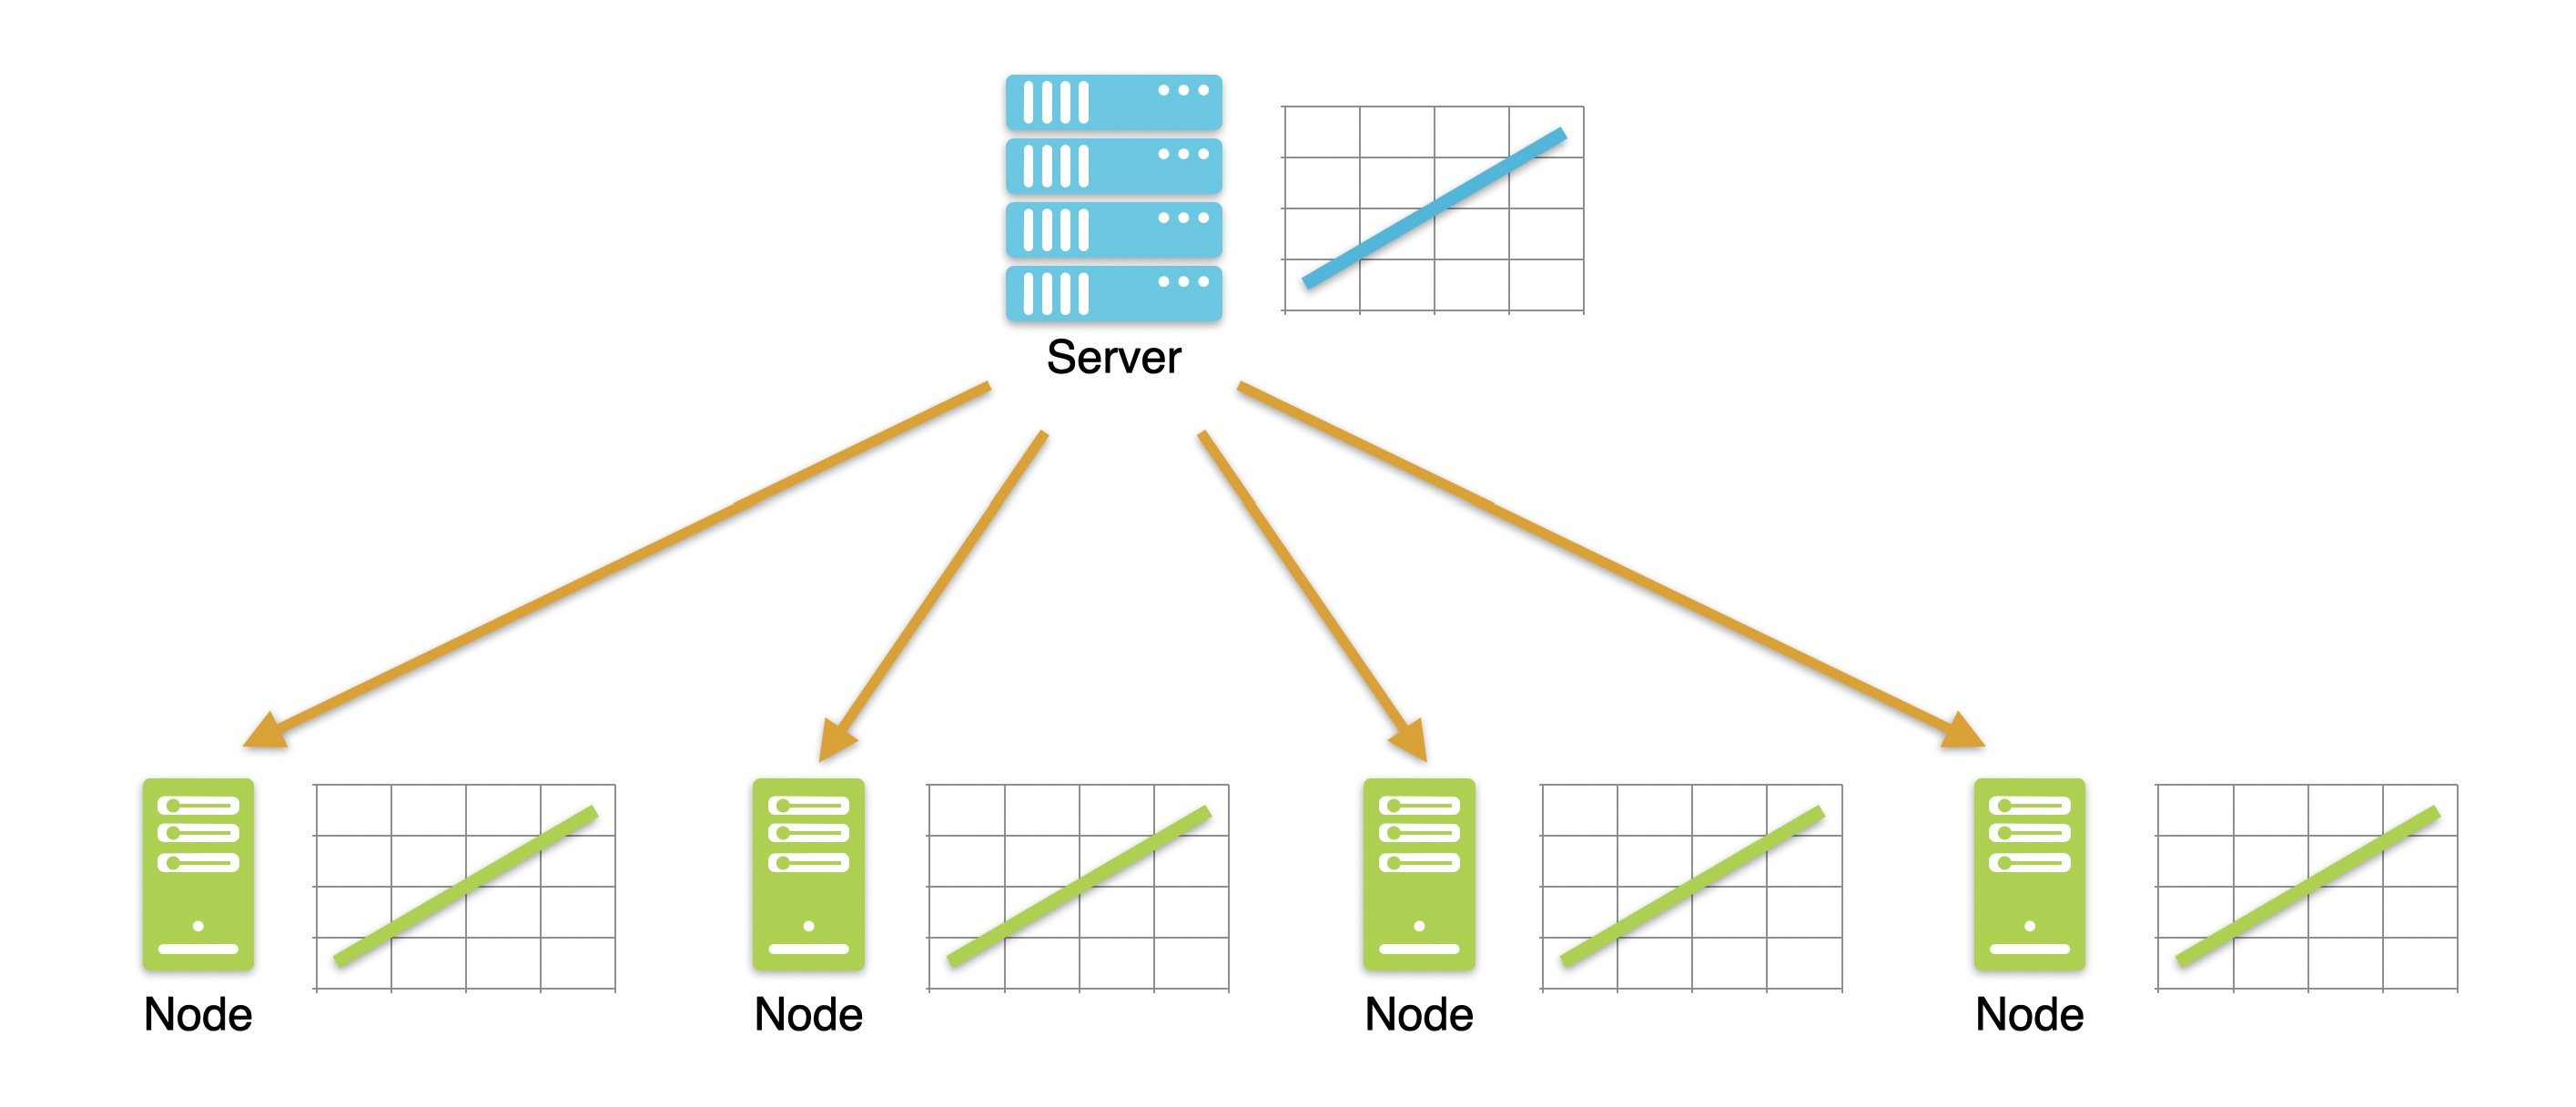
\includegraphics[width=\linewidth]{FL-phase1.jpg}
    \vspace*{-.8cm}
    \caption{First distribution of the model, from the server to the participating nodes}
    \label{fig:fl-phase1}
\end{figure}

\begin{figure}[t]
    \centering
    \vspace*{-.4cm}
    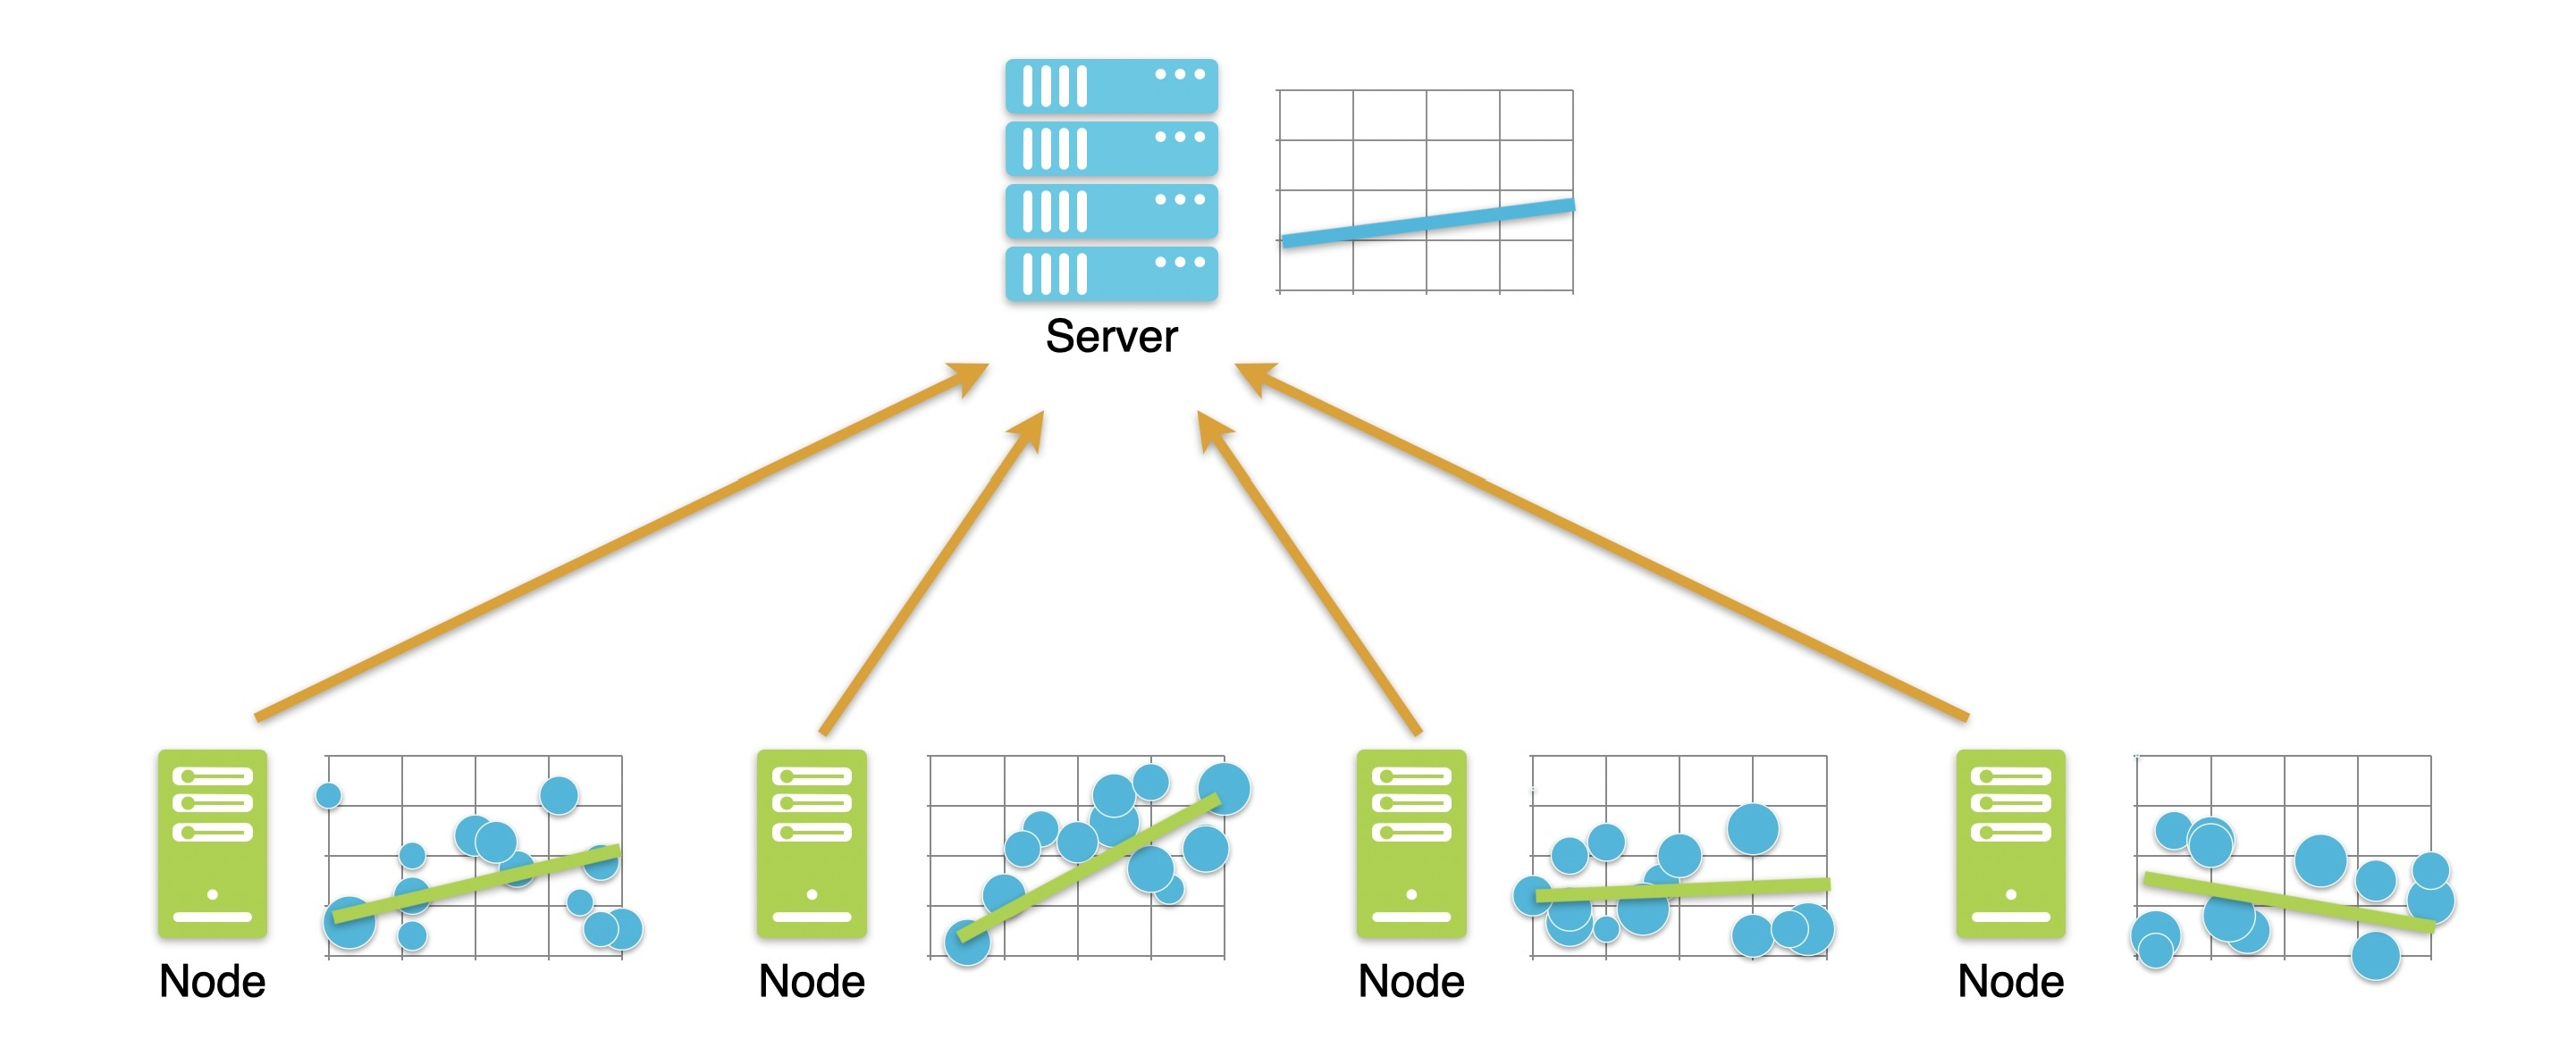
\includegraphics[width=\linewidth]{FL-phase2.jpg}
    \vspace*{-.8cm}
    \caption{Models modified by nodes, by integrating local data, are returned to the server}
    \label{fig:fl-phase2}
\end{figure}

Despite its promising potential, \gls{fl} faces several challenges, including power consumption, dropped connections or high-latency due to stragglers.
Moreover, other issues must be considered, like communication overhead and privacy concerns. % such as man-in-the-middle attacks.
These challenges necessitate robust solutions like end-to-end encryption and secure aggregation to safeguard data integrity and confidentiality.

%% DIFFERENT APPROACH OF FL
\subsection{Different Approaches of \gls{fl}}

Two variations of \gls{fl} exists, which are tailored to different contexts and requirements: \gls{cdfl} and \gls{csfl}.

\paragraph*{Cross-device FL} In \emph{cross-device} settings, the participating devices are typically heterogeneous and widely distributed, encompassing a massive number of parties, such as smartphones, IoT devices, and personal computers, potentially ranging from thousands to billions, with each device possessing a small dataset.
Due to the diversity of devices and their varying computational capabilities, cross-device \gls{fl} often encounters challenges related to limited availability, reliability, and communication overhead, but offers scalability and adaptability, making it suitable for scenarios where a large and diverse set of devices collaborate on model training tasks.

\paragraph*{Cross-silo FL} In contrast, \emph{cross-silo} \gls{fl} operates within organizational boundaries or distinct data silos, where each silo represents a separate entity or institution.
Silos could correspond to different departments within a company, independent organizations, or even geographical regions.
Unlike \gls{cdfl}, which involves heterogeneous devices, \gls{csfl} typically implies organization with more homogeneous capabilities and more data to train on.
Parties in cross-silo \gls{fl} are more likely to be reliable and consistently available for participation, as they are usually institutional entities with dedicated infrastructure and resources.
Yet, entities involved in \gls{csfl} also tend to have considerably greater discrepancies in terms of objectives and data-distributions, and sometimes even model architectures.
Cross-silo \gls{fl} offers more control over data governance and security, as data sharing occurs within predefined organizational boundaries, facilitating compliance with regulatory requirements and privacy policies.
%\end{itemize}

On the other side, two paradigms of distribution exist in the federated approach, each offering unique advantages and challenges, catering to different use cases and requirements.


%\begin{itemize}
\paragraph*{Server-orchestrated FL} 
A central server coordinates the training process by managing communication between participating devices and aggregating model updates. The central server plays a pivotal role in distributing model parameters, orchestrating training rounds, and aggregating updates from individual devices. This approach requires global coordination and synchronization, as all communication and aggregation activities are orchestrated by the server. While server-orchestrated \gls{fl} offers centralized control and streamlined management, it also introduces potential single points of failure and scalability limitations due to the server's central role.

\paragraph*{Fully decentralized FL}
There is no central server orchestrating the training process. Instead, devices communicate directly with each other and perform local model updates and aggregations independently. Each device acts autonomously, making decisions regarding model training, aggregation, and synchronization without reliance on a central authority. This decentralized approach eliminates single points of failure and allows for greater scalability, as communication and computation can be distributed across a large number of devices.
However, fully decentralized \gls{fl} may face challenges related to coordination, consistency, and synchronization, especially in scenarios with a vast number of participating devices.
%\end{itemize}

%% WIDE ACCEPTANCE OF THE PARADIGM 
\subsection{Wide Acceptance of the Paradigm}

As evidenced by its exponential growth in research (from a few dozens in the first years to thousands of publications today) and real-world deployments, \gls{fl} stands as a burgeoning field with profound implications for various industries. With open-source libraries like PySyft and TensorFlow Federated facilitating its adoption, \gls{fl} fosters interdisciplinary collaboration, bridging machine learning, privacy, and networked systems to shape the future of decentralized intelligence.


\section{Federated Learning for Collaborative Network Security} % Léo
\label{sec:fids}

%% AI in network security
% The increasingly complex and heterogeneous nature of network environments has necessitated the deployment of \gls{ai} and \gls{ml} techniques to properly detect and mitigate security threats. 
% In this context, \gls{ai} can intervene at various stages of the network security lifecycle, from threat detection (\eg, \glspl{ids}) to alert correlation and triage (\eg, in \glspl{siem}).
% \Glspl{ai}-enriched \glspl{ids} have emerged as a critical component of modern network security architectures, enabling organizations to timely detect security incidents.
% \Gls{dl} techniques, in particular, have shown promising results in enhancing the performance of \glspl{ids} by allowing for learning more complex patterns and behaviors, and generalizing to zero- or one-day attacks.

\Gls{ai} can intervene at various stages of the network security lifecycle, from threat detection to alert correlation and triage.
%In particular, \glspl{ai}-enriched \glspl{ids} have emerged as a critical component of modern network security architectures, enabling organizations to timely detect security incidents.
\Gls{dl} techniques, in particular, have shown promising results in enhancing the performance of \glspl{ids} by allowing for learning more complex patterns and behaviors, and generalizing to zero- or one-day attacks.
%% FL for intrusion detection
Yet, training \gls{dl}-based \glspl{ids} requires large amounts of labeled data to properly learn the underlying patterns of normal and malicious behaviors.
In practice, organizations often face challenges in collecting and sharing such data due to privacy concerns, such as sensitive information leakage or regulatory compliance.
\Gls{fl} offers a compelling solution to this problem by enabling organizations to collaboratively train \gls{ids} models without sharing raw data.

%% CIDS / FIDS
Typical \gls{fl} applications often imply cross-device settings, with the hypothesis of a single actor trying to learn from multiple devices without accessing their data.
The \gls{cids} use case is slightly different, as it usually involves multiple organizations, each owning independent datasets and infrastructures.
We refer to \gls{cids} leveraging \gls{fl} as \gls{fids}, as they are federated across organizations.
%
%% Data heterogeneity
This context raises new challenges, notably the heterogeneity of the data distributions across organizations.
These differences can further vary in terms of monitored traffic (\eg, services, protocols, user behavior), the deployed security solutions, or even the \gls{dl} models used.
The last point is particularly critical, as it prevents the direct aggregation of models as done by \texttt{FedAvg}~\cite{mcmahan_communication-efficient_2017}.

Simplifying the problem, we can consider the case of a shared model architecture, ensuring the applicability of most \gls{fl} strategies.
Yet, the data heterogeneity remains a significant challenge, as model aggregation of highly heterogeneous data is already identified as an open challenge in \gls{fl} literature~\cite{zhu_federated_2021}.

%% Sota
Previous works~\cite{lavaur_evolution_2022} provided a comprehensive overview of the state-of-the-art of \glspl{fids}, identifying clear research directions.
These challenges span over three main axes:

\begin{enumerate}[(i)]
    \item \emph{Transferability, adaptability, and scalability.}
    How to deal with a high number of clients and constrained environments?
    How to learn from heterogeneous data, or heterogeneous clients?
    How to balance generalization and specialization for model aggregation?

    \item \emph{Security, trust, and resilience.}
    How to resist to poisoning and inference attacks against the aggregated models?
%    How to protect sharing and aggregation?
    How to deal with untrusted or malicious participants?
    How to leverage \gls{fl} to react to attacks?

    \item \emph{Local algorithm and aggregation performance.}
    What is the impact of the hyper- and meta-parameters?
    How to model behaviors to better characterize traffic?
    How to improve the raw performance of models?
\end{enumerate}


\section{Security Challenges in Federated Learning} % Léo
\label{sec:threats}

%% Threats against FL in IDS context
% - against the model
% - against privacy
The distributed nature of \gls{fids} opens the way to various attack vectors, ranging from poisoning attacks to privacy breaches.
The former aim at altering the global model's behavior, while the latter target the confidentiality of the data used by the participants' in training.
We especially focus on the poisoning attacks, as they are particularly relevant in the context of \gls{fids}~\cite{lavaur_icdcs_demo}.
Indeed, the ability to manipulate the global model is a significant threat, as it can lead to an overall decrease in the protected system's security.
\citet{rodriguez-barroso_survey_2023} summarizes the different types of poisoning attacks in a fourfold taxonomy:

\begin{enumerate}[(i)]
\item \emph{Attack Moment}: whether the attack is performed during the training or the inference phase.

\item \emph{Attackers' Objective}: Targeted/Backdoor attacks aim at specific samples or classes, modifying the model's behavior when subjected to specific behaviors, while untargeted poisoning alters the global model uniformly.

\item \emph{Poisoned components}: depending on if the attacks alters the training data or the model directly, the impact will vary.

\item \emph{Frequency}: one-shot attacks or adaptive/iterative ones.
    In the latter case, different strategies can be adopted, \eg, increasing the percentage data over time to slowly divert the global model of its original local optimum.
\end{enumerate}

\subsection{Threat modeling in FL settings}

%% Different threat models
Depending on the attacker's positioning and knowledge, different threat models can be considered.
%\begin{enumerate}

    \paragraph*{Outsider \vs Insider}
    An outsider has no knowledge of the model or the data used and cannot interact with the system, while an insider has access to the model and its own local data.
    Further, insiders can impact the model's behavior, and therefore the other participants, while outsiders are limited to listening to the communication channel.
    
    \paragraph*{Lone \vs Colluding Attackers}
    Especially in the context of insiders, attackers can act alone or in collusion to maximize their impact.
    This collusion can be caused by a single entity controlling clients (Sybils) or multiple entities sharing a common interest.
    
    \paragraph*{Honest-but-curious \vs malicious clients}
    Honest-but-curious clients follow the protocol but try to learn from the model or the data, while malicious clients actively try to disrupt the system.
%\end{enumerate}

%% Attack taxonomy


%% Mitigation strategies

\subsection{Mitigation strategies}

Fortunately, the community also proposed numerous mitigation strategies against adversarial attacks targeting \gls{fl} systems, and \gls{fids} by extension.
Specifically, multiple works have focused on the development of robust aggregation algorithms and contributions filtering mechanisms, which can mitigate the effect of poisoning attacks.
These strategies can be classified into three main categories:

%\begin{enumerate}
\paragraph*{Server-side evaluation} the server evaluates the received contributions on a purpose-built representative dataset.
This is mostly inapplicable in \gls{niid} settings, as building a representative dataset would imply having access to the clients' data-distribution.
    
\paragraph*{Server-side model comparison} the server compares the received contributions to a reference model, or to each other.
In the former, just as in the previous case, the absence of a single-source-of-truth in \gls{niid} settings makes this approach difficult.
By comparing models to each other, however, the server can detect discrepancies and identify potential malicious contributions.
This is the strategy leveraged by \texttt{FoolsGold}~\cite{fung_limitations_2020} or \texttt{FLAME}~\cite{nguyen_flame_2022}, although with different approaches and objectives.

\paragraph*{Client-side evaluation} the clients are tasked to evaluate other participants' contributions and generate metrics using their local dataset.
This removes the need for a single source of truth, while the metrics act as feedbacks that can be used to feed reputation systems.
%\end{enumerate}



\section{Conclusion} % Yann
\glsresetall

%In conclusion, this article has provided a comprehensive overview of \gls{fl} and its applications in collaborative network security. Through hands-on tutorials and discussions, participants have gained valuable insights into the fundamental principles of \gls{fl}, its practical implementation using the Flower framework, and its role in training Collaborative Intrusion Detection Systems (CIDS). As organizations increasingly rely on decentralized data sources for model training, \gls{fl} emerges as a powerful solution for aggregating knowledge while preserving data privacy. However, the deployment of Federated Intrusion Detection Systems (FIDS) brings forth unique security challenges, including the threat of poisoning attacks. By equipping participants with the knowledge and tools to address these challenges, this tutorial aims to empower researchers and practitioners in harnessing the full potential of \gls{fl} for collaborative network security. Looking ahead, further research and development efforts will be crucial in advancing \gls{fl} techniques and enhancing the resilience of \gls{fl} systems against emerging threats in distributed computing environments.


In conclusion, this article has covered the fundamentals of \gls{fl} and its applications in collaborative network security. Participants gained insights into \gls{fl} principles, practical implementation (using the Flower framework), and its role in training \gls{cids}. \gls{fl} offers a powerful solution for decentralized data training while preserving privacy. However, deploying \gls{fids} poses unique security challenges, such as poisoning attacks. By providing knowledge and tools to tackle these challenges, this tutorial aims to empower researchers and practitioners in utilizing \gls{fl} for collaborative network security. Moving forward, further research and development efforts are essential to advance \gls{fl} techniques and enhance the resilience of \gls{fl} systems against emerging threats in distributed computing environments.


\printbibliography

\end{document}